\documentclass[conference]{IEEEtran}

\usepackage{cite}
\usepackage{amsmath,amssymb,amsfonts}
\usepackage{algorithmic}
\usepackage{graphicx}
\usepackage{textcomp}
\usepackage{xcolor}
\usepackage{booktabs}
\usepackage{multirow}
\usepackage{hyperref}
\usepackage{float}

\begin{document}

\title{When Does Focal Loss Help? A Controlled Comparison of Focal Loss and
Cross-Entropy for Small-CNN Image Classification on Balanced and Long-Tailed CIFAR-10}

\author{
\IEEEauthorblockN{Naman Dwivedi\IEEEauthorrefmark{1},
Raj Dandekar\IEEEauthorrefmark{1},
Rajat Dandekar\IEEEauthorrefmark{1},
Sreedath Panat\IEEEauthorrefmark{1}}
\IEEEauthorblockA{\IEEEauthorrefmark{1}Vizuara AI Labs, hello@vizuara.com}
}

\maketitle

\begin{abstract}
Focal loss was introduced to address foreground-background imbalance in dense object
detection, yet it is often adopted as a generic drop-in replacement for cross-entropy in
image classification. We ask a precise question: does focal loss beat cross-entropy for
CIFAR-10 classification with a small convolutional neural network? Holding a 0.31M-parameter
CNN, optimizer, schedule, and data augmentation fixed, we vary only the loss function
(cross-entropy versus focal loss with $\gamma \in \{1,2,3\}$) and the class distribution
(balanced CIFAR-10 versus long-tailed CIFAR-10-LT with imbalance factor 100), and we report
top-1 accuracy, Expected Calibration Error (ECE), macro-F1, and worst-class accuracy. On
balanced CIFAR-10, cross-entropy attains the best accuracy (87.90\%); focal loss never
exceeds it and degrades monotonically with $\gamma$, its only benefit being improved
calibration at $\gamma=1$ (ECE 0.0154 versus 0.0337). Under class imbalance the conclusion
reverses: focal loss with $\gamma=3$ improves accuracy (59.10\% versus 57.66\%), macro-F1
(by 3.2 points), worst-class accuracy (3.6\% to 13.3\%, a 3.7$\times$ gain), and calibration
(ECE 0.220 to 0.050). We conclude that focal loss is a tool for imbalance and calibration,
not a generic accuracy upgrade, and we provide practical guidance on selecting $\gamma$.
All code and results are released.
\end{abstract}

\begin{IEEEkeywords}
focal loss, cross-entropy, image classification, class imbalance, model calibration, CIFAR-10
\end{IEEEkeywords}

\section{Introduction}
The choice of loss function is among the most consequential decisions when training a
classifier. Softmax cross-entropy is the default for image classification, but a steady stream
of alternatives promises improvements on specific failure modes. Focal loss~\cite{lin2017focal}
is one of the most widely adopted: by multiplying the cross-entropy term with a modulating
factor that down-weights well-classified examples, it was designed to combat the extreme
foreground-background imbalance encountered in one-stage dense object detection.

Because of its success in detection, focal loss is frequently reused as a generic replacement
for cross-entropy in classification tasks, often without verifying that the conditions that
made it effective are present. This motivates a precise and falsifiable question: \emph{does
focal loss beat cross-entropy for CIFAR-10 classification with a small CNN?} CIFAR-10 is a
balanced benchmark, so a priori there is little of the easy-example dominance that focal loss
is designed to suppress.

We answer this question with a tightly controlled study. We fix a small convolutional network,
its optimizer, learning-rate schedule, and data augmentation, and vary only two factors: the
loss function (cross-entropy versus focal loss with $\gamma \in \{1,2,3\}$) and the class
distribution (the standard balanced CIFAR-10 versus a long-tailed variant, CIFAR-10-LT, with
imbalance factor 100). Figure~\ref{fig:design} summarizes the design. We evaluate four
complementary metrics: top-1 accuracy, Expected Calibration Error (ECE), macro-F1, and
worst-class accuracy.

\noindent\textbf{Contributions.}
\begin{itemize}
\item A clean, fully reproducible head-to-head comparison of cross-entropy and focal loss
($\gamma \in \{1,2,3\}$) on balanced and long-tailed CIFAR-10 with a single fixed small CNN.
\item Evidence that on balanced data cross-entropy wins on accuracy and focal loss helps only
calibration, and only at low $\gamma$.
\item Evidence that under class imbalance the verdict reverses on every metric, with larger
$\gamma$ preferred, and a 3.7$\times$ improvement in worst-class accuracy.
\item Practical guidance on when to use focal loss, with open code and results executed on
serverless GPUs.
\end{itemize}

The remainder of the paper reviews related work (Section~\ref{sec:related}), formalizes the
losses and metrics (Section~\ref{sec:method}), details the experimental setup
(Section~\ref{sec:setup}), presents results (Section~\ref{sec:results}), and discusses
limitations (Section~\ref{sec:limits}) and conclusions (Section~\ref{sec:conclusion}).

\begin{figure}[t]
\centering
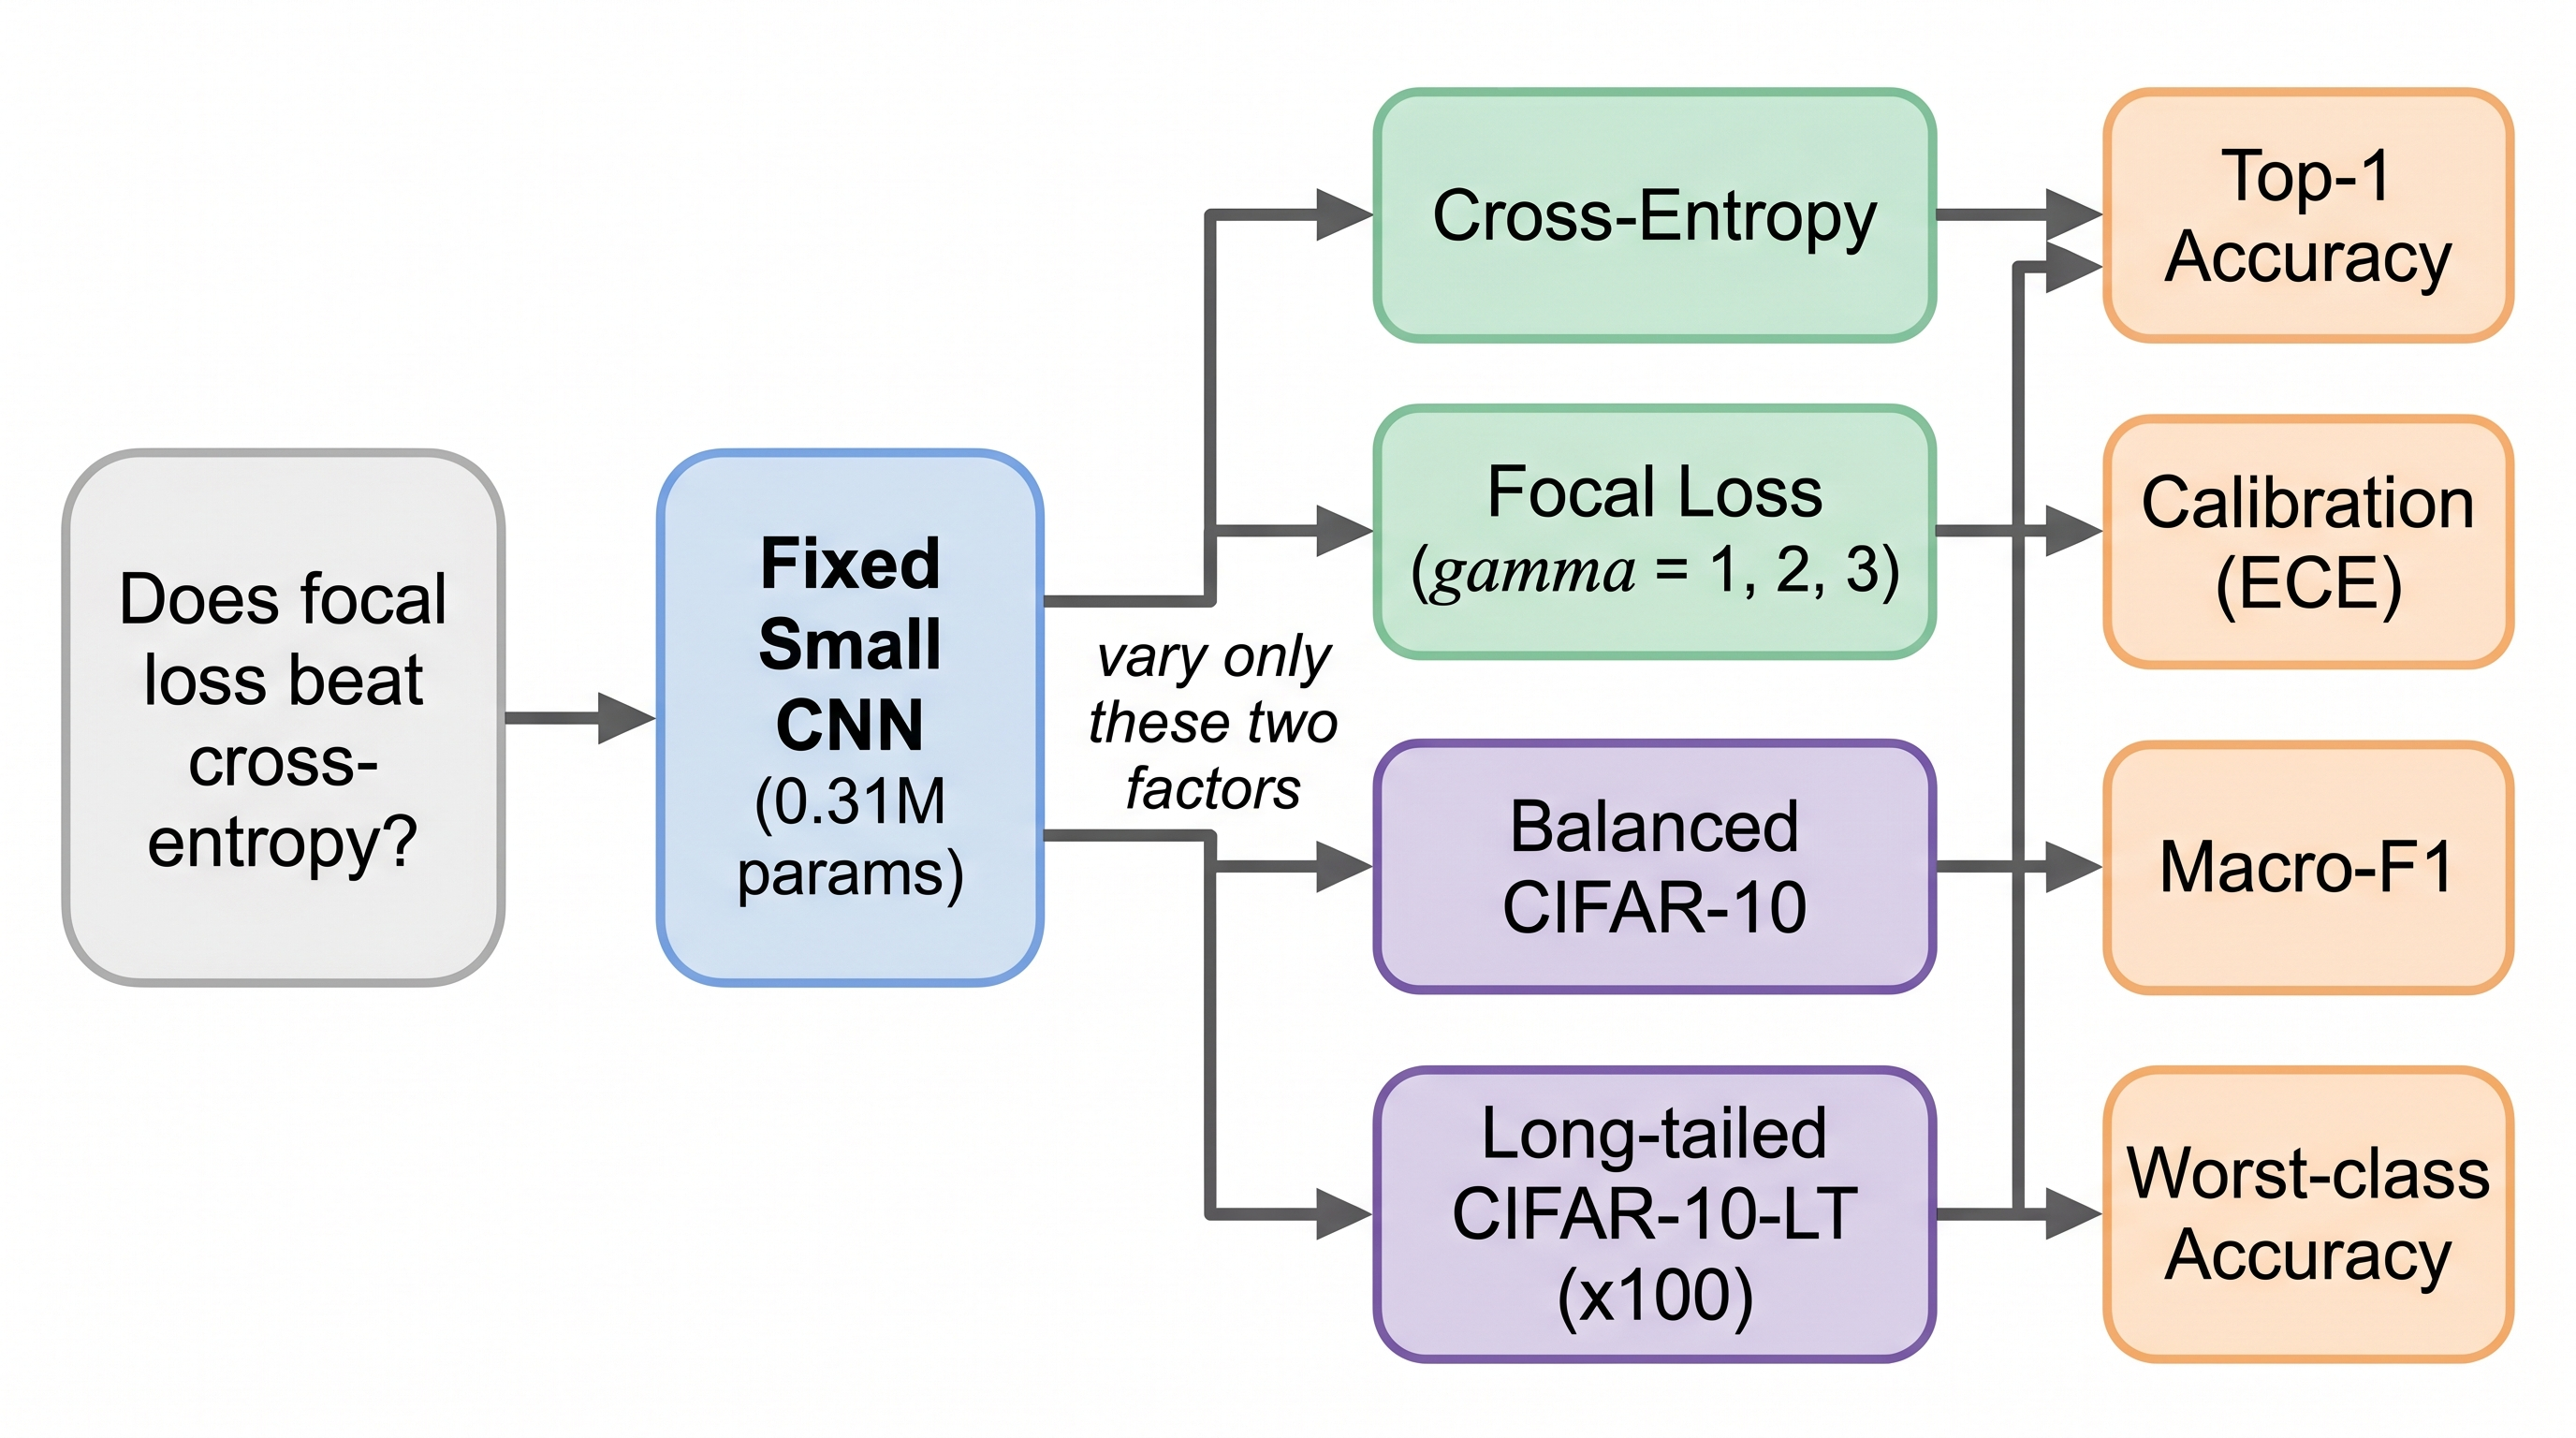
\includegraphics[width=\columnwidth]{figures/output/fig1_design.png}
\caption{Controlled experimental design. Only the loss function and the class distribution are
varied; the model, optimizer, schedule, and augmentation are held fixed. Each configuration is
evaluated on four metrics.}
\label{fig:design}
\end{figure}

\section{Background and Related Work}
\label{sec:related}

\subsection{Focal Loss and Class Imbalance}
Focal loss~\cite{lin2017focal} reshapes cross-entropy to focus training on hard examples and
was central to the RetinaNet detector. In long-tailed recognition, reweighting and margin-based
methods are the dominant tools: the Class-Balanced loss~\cite{cui2019classbalanced} reweights by
the effective number of samples and, in its CB-Focal form, improves on plain focal loss under
imbalance; LDAM~\cite{cao2019ldam} enforces label-distribution-aware margins. These works
establish focal loss as a baseline for imbalance rather than a general-purpose accuracy method.

\subsection{Calibration of Neural Networks}
Modern networks are often miscalibrated, tending to be overconfident~\cite{guo2017calibration}.
Mukhoti et al.~\cite{mukhoti2020calibration} show that focal loss produces substantially better
calibrated classifiers than cross-entropy without sacrificing accuracy, and that combining it
with temperature scaling yields state-of-the-art calibration. Their analysis predicts a
calibration benefit even on balanced data, which our experiments test directly.

\subsection{Long-Tailed Recognition Benchmarks}
Long-tailed CIFAR variants, constructed by exponentially subsampling classes, are a standard
testbed for imbalance~\cite{cui2019classbalanced,buda2018systematic}. We adopt the same
construction with an imbalance factor of 100.

\section{Methodology}
\label{sec:method}

\subsection{Problem Formulation}
For an input with ground-truth class $y$ and predicted class probabilities $p$, let
$p_t = p_y$ denote the probability assigned to the true class. Softmax cross-entropy is
\begin{equation}
\mathcal{L}_{\mathrm{CE}} = -\log(p_t).
\end{equation}
Focal loss~\cite{lin2017focal} introduces a modulating factor with focusing parameter
$\gamma \geq 0$:
\begin{equation}
\mathcal{L}_{\mathrm{FL}} = -(1 - p_t)^{\gamma}\,\log(p_t).
\end{equation}
When $\gamma = 0$, focal loss reduces exactly to cross-entropy; as $\gamma$ increases, the loss
contributed by easy, well-classified examples ($p_t \to 1$) is increasingly suppressed. We use
the multi-class form with $\gamma \in \{1, 2, 3\}$ and probabilities clamped to $[10^{-7}, 1]$
for numerical stability.

\subsection{Small CNN Architecture}
We use a compact convolutional network (Fig.~\ref{fig:arch}) of three convolutional blocks with
32, 64, and 128 channels. Each block applies two Conv-BatchNorm-ReLU units followed by
$2\times2$ max pooling. A global average pool feeds a fully connected layer of width 128 with
dropout 0.3 and a final linear classifier over the ten classes. The network has 305{,}706
trainable parameters. The hyperparameters are listed in Table~\ref{tab:hparams}.

\begin{figure}[t]
\centering
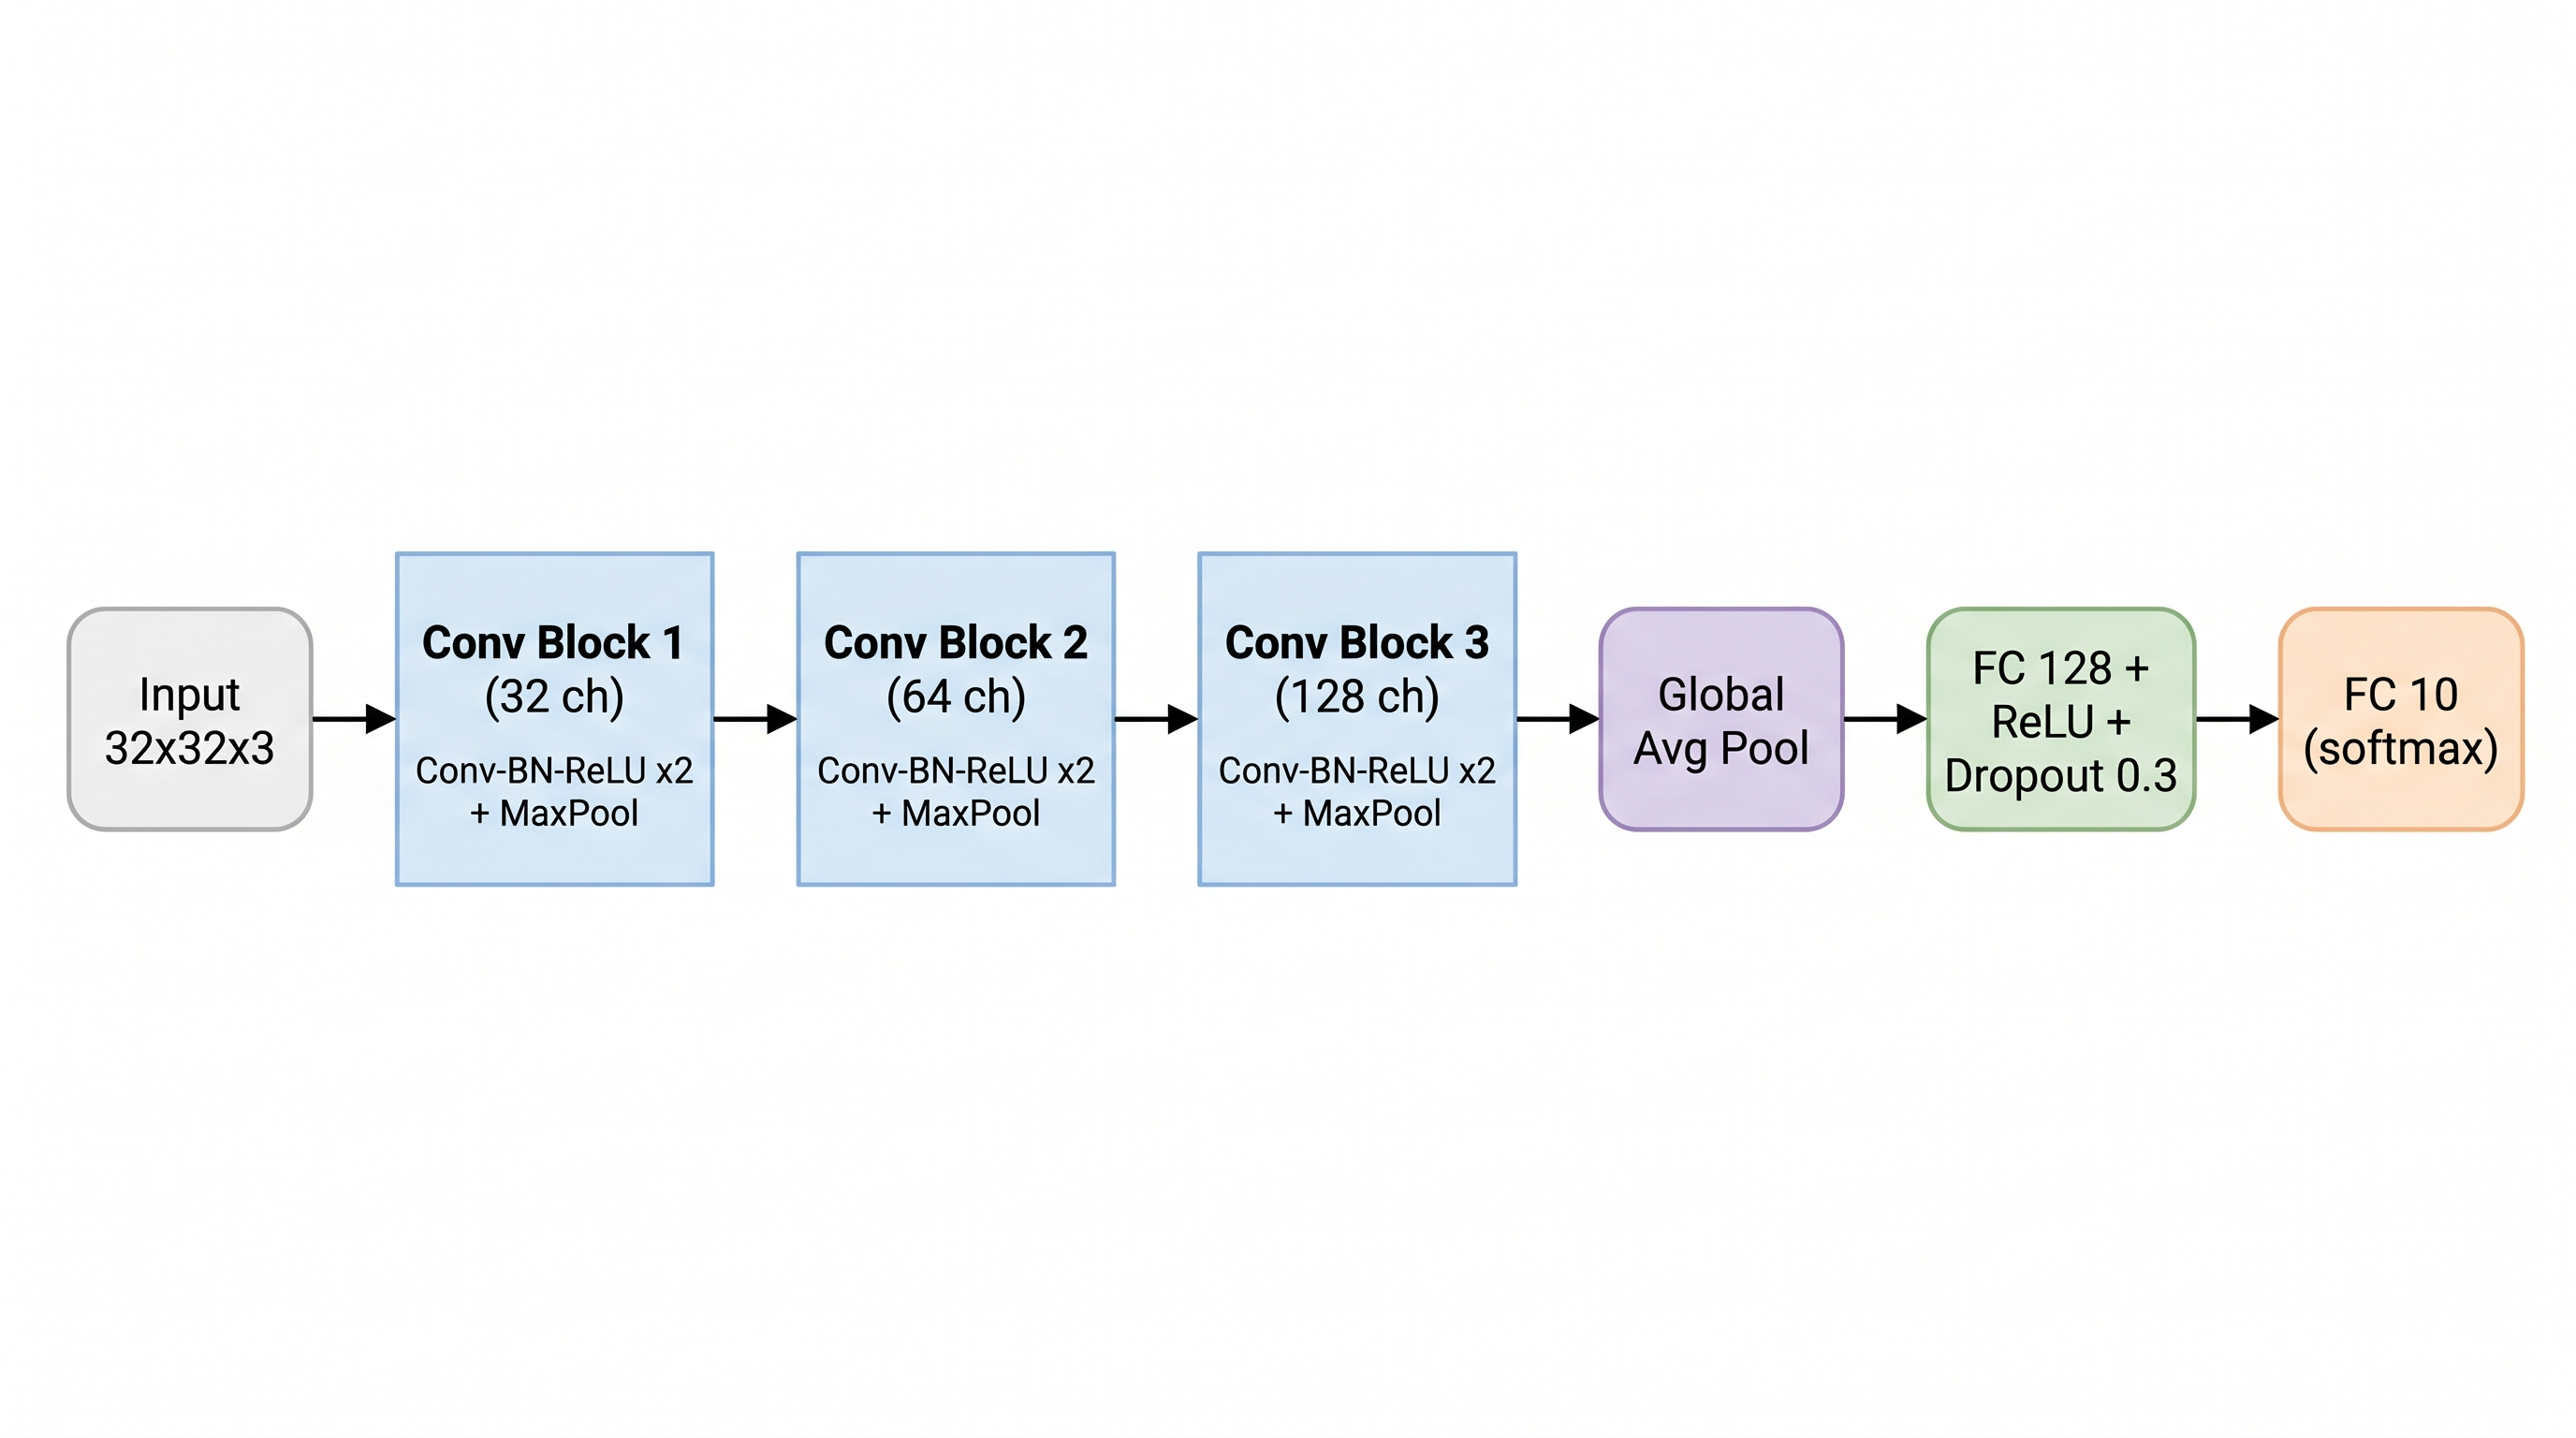
\includegraphics[width=\columnwidth]{figures/output/fig2_architecture.png}
\caption{The fixed 0.31M-parameter small CNN used in all experiments: three convolutional
blocks followed by global average pooling and a compact classifier head.}
\label{fig:arch}
\end{figure}

\begin{table}[t]
\caption{Architecture and Training Hyperparameters}
\label{tab:hparams}
\centering
\begin{tabular}{ll}
\toprule
\textbf{Setting} & \textbf{Value} \\
\midrule
Parameters & 305{,}706 \\
Optimizer & AdamW (lr $10^{-3}$, weight decay $5\times10^{-4}$) \\
Schedule & Cosine annealing \\
Epochs & 30 \\
Batch size & 128 \\
Augmentation & RandomCrop(32, pad 4), horizontal flip \\
Dropout & 0.3 \\
Hardware & Modal serverless NVIDIA A100-40GB \\
Framework & PyTorch 2.4 \\
\bottomrule
\end{tabular}
\end{table}

\subsection{Long-Tailed Data Construction}
To probe the imbalanced regime we build CIFAR-10-LT by subsampling the training set so that the
number of examples per class follows an exponential profile. For class index
$c \in \{0,\dots,9\}$ and imbalance factor $\rho$,
\begin{equation}
n_c = n_{\max}\,\rho^{-c/(C-1)},
\end{equation}
with $n_{\max} = 5000$, $C = 10$, and $\rho = 100$, giving per-class counts
$[5000, 2997, 1797, 1077, 646, 387, 232, 139, 83, 50]$. The test set remains balanced.

\subsection{Evaluation Metrics}
We report top-1 accuracy; macro-F1 (the unweighted mean of per-class F1, which exposes tail
performance); worst-class accuracy (the minimum per-class accuracy); and the Expected
Calibration Error with $M=15$ equal-width confidence bins,
\begin{equation}
\mathrm{ECE} = \sum_{m=1}^{M} \frac{|B_m|}{N}\,\bigl|\,\mathrm{acc}(B_m) - \mathrm{conf}(B_m)\,\bigr|,
\end{equation}
where $B_m$ is the set of predictions whose confidence falls in bin $m$.

\section{Experimental Setup}
\label{sec:setup}

\subsection{Datasets}
We use the standard CIFAR-10 dataset (50{,}000 training and 10{,}000 test images, $32\times32$
RGB, ten balanced classes) and the long-tailed CIFAR-10-LT variant described above
(approximately 12{,}408 training images, balanced test set).

\subsection{Implementation Details}
All runs use the architecture and hyperparameters of Table~\ref{tab:hparams}, executed on Modal
serverless A100-40GB GPUs with a fixed random seed. Each run trains for 30 epochs in roughly two
to four minutes; the full study used about twenty minutes of GPU time.

\subsection{Compared Configurations}
On balanced CIFAR-10 we compare cross-entropy against focal loss with $\gamma \in \{1,2,3\}$. On
CIFAR-10-LT we compare cross-entropy against focal loss with $\gamma \in \{2,3\}$, the settings
expected to be most effective under imbalance.

\section{Results}
\label{sec:results}

\subsection{Balanced CIFAR-10}
Table~\ref{tab:balanced} and Fig.~\ref{fig:balanced} report the balanced results. Cross-entropy
achieves the best top-1 accuracy (87.90\%). Focal loss does not exceed it at any $\gamma$, and
accuracy decreases monotonically as $\gamma$ grows (87.44\%, 87.28\%, 86.38\%). The one benefit
of focal loss appears in calibration: at $\gamma = 1$ it more than halves the ECE relative to
cross-entropy (0.0154 versus 0.0337). However, at $\gamma \geq 2$ the calibration error exceeds
that of cross-entropy, as the strong down-weighting makes the model underconfident. On balanced
data, therefore, the only advantage of focal loss is improved calibration, and only at low
$\gamma$.

\begin{table}[t]
\caption{Balanced CIFAR-10 Results (Small CNN, 30 Epochs)}
\label{tab:balanced}
\centering
\begin{tabular}{lcccc}
\toprule
\textbf{Loss} & \textbf{Acc} & \textbf{ECE} & \textbf{Macro-F1} & \textbf{Worst-cls} \\
\midrule
\textbf{Cross-entropy} & \textbf{0.8790} & 0.0337 & \textbf{0.8786} & 0.729 \\
Focal $\gamma=1$ & 0.8744 & \textbf{0.0154} & 0.8741 & \textbf{0.743} \\
Focal $\gamma=2$ & 0.8728 & 0.0660 & 0.8724 & 0.715 \\
Focal $\gamma=3$ & 0.8638 & 0.1096 & 0.8632 & 0.692 \\
\bottomrule
\end{tabular}
\end{table}

\begin{figure}[t]
\centering
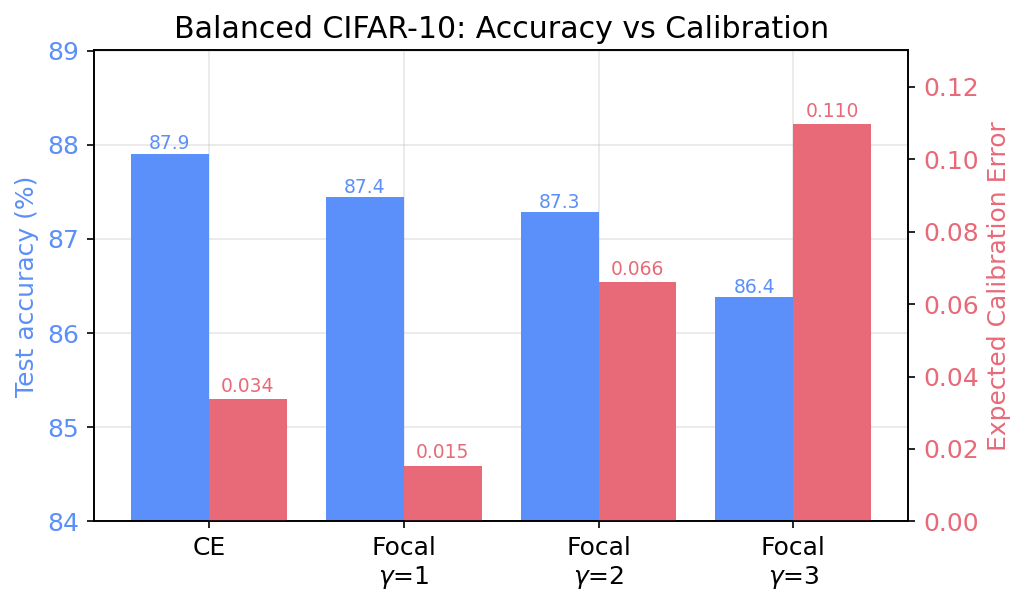
\includegraphics[width=\columnwidth]{figures/output/fig3_balanced.png}
\caption{On balanced CIFAR-10, cross-entropy yields the best accuracy while focal loss with
$\gamma=1$ yields the best calibration; larger $\gamma$ degrades both accuracy and calibration.}
\label{fig:balanced}
\end{figure}

\subsection{Long-Tailed CIFAR-10-LT}
Table~\ref{tab:imbalanced} and Fig.~\ref{fig:imbalanced} report the imbalanced results. Here the
verdict reverses: focal loss improves on cross-entropy across all metrics, and larger $\gamma$
helps more. At $\gamma = 3$, accuracy rises from 57.66\% to 59.10\%, macro-F1 from 0.5332 to
0.5655, and ECE falls from 0.2202 to 0.0503. The most striking effect is on the rarest classes:
worst-class accuracy increases from 3.6\% to 13.3\%, a 3.7$\times$ improvement.
Figure~\ref{fig:perclass} plots per-class accuracy ordered by training frequency and shows that
the gains are concentrated in the tail, where cross-entropy collapses while focal loss preserves
a meaningful fraction of accuracy. Figure~\ref{fig:curves} shows the training dynamics.

\begin{table}[t]
\caption{Long-Tailed CIFAR-10-LT Results (Imbalance Factor 100)}
\label{tab:imbalanced}
\centering
\begin{tabular}{lcccc}
\toprule
\textbf{Loss} & \textbf{Acc} & \textbf{ECE} & \textbf{Macro-F1} & \textbf{Worst-cls} \\
\midrule
Cross-entropy & 0.5766 & 0.2202 & 0.5332 & 0.036 \\
Focal $\gamma=2$ & 0.5908 & 0.0967 & 0.5618 & 0.114 \\
\textbf{Focal $\gamma=3$} & \textbf{0.5910} & \textbf{0.0503} & \textbf{0.5655} & \textbf{0.133} \\
\bottomrule
\end{tabular}
\end{table}

\begin{figure}[t]
\centering
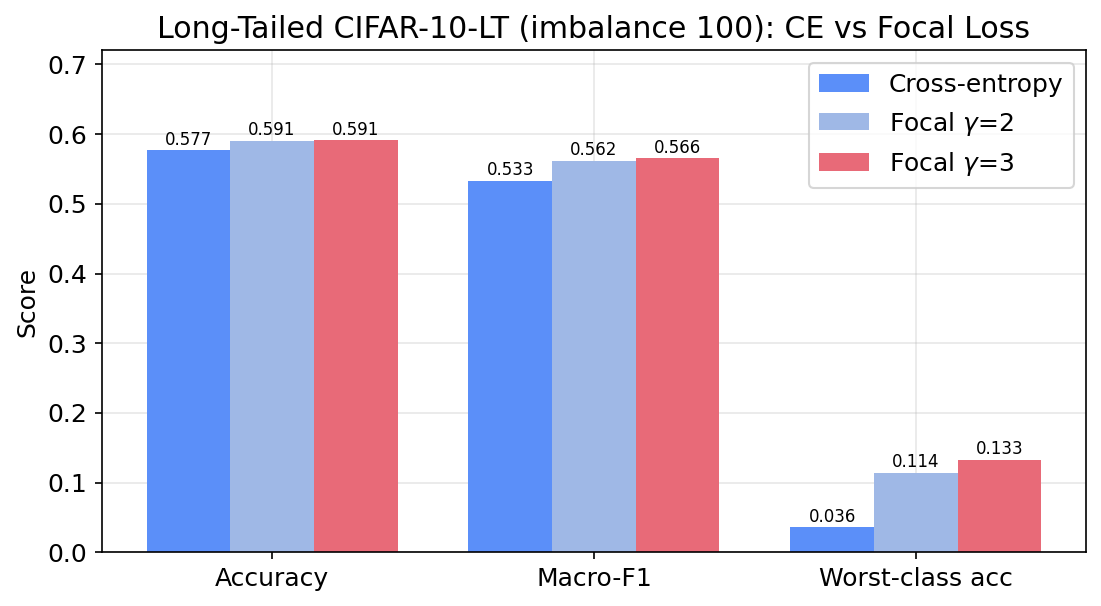
\includegraphics[width=\columnwidth]{figures/output/fig4_imbalanced.png}
\caption{Under imbalance (factor 100), focal loss improves accuracy, macro-F1, and especially
worst-class accuracy over cross-entropy.}
\label{fig:imbalanced}
\end{figure}

\begin{figure}[t]
\centering
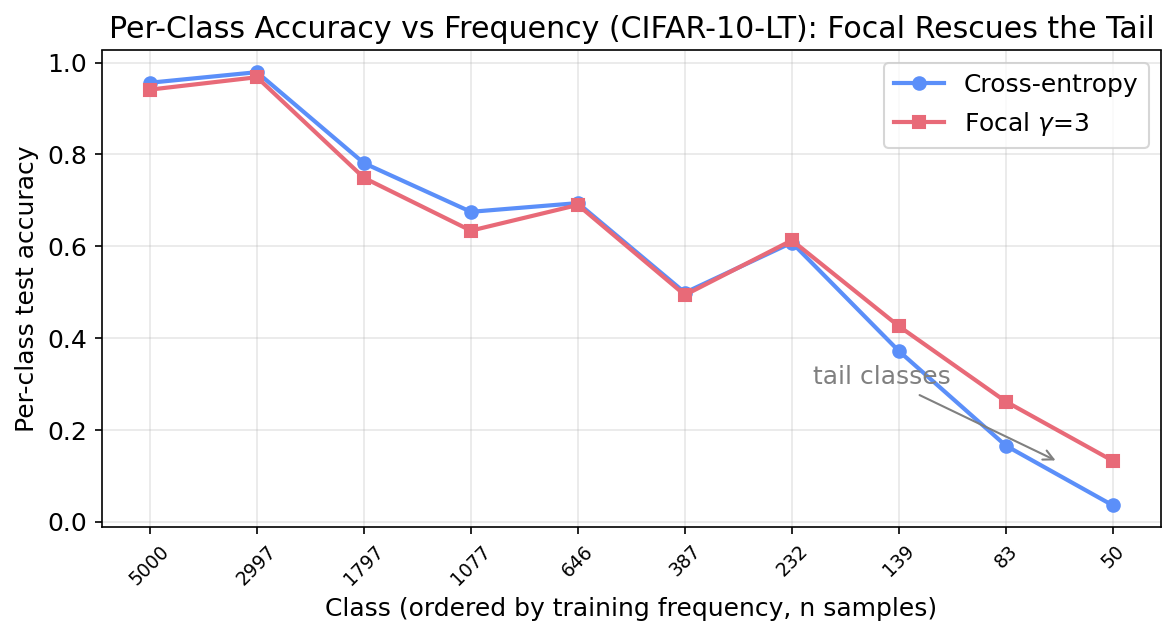
\includegraphics[width=\columnwidth]{figures/output/fig5_perclass.png}
\caption{Per-class accuracy ordered by training frequency on CIFAR-10-LT. Focal loss
($\gamma=3$) recovers accuracy on the rarest classes (right) where cross-entropy collapses.}
\label{fig:perclass}
\end{figure}

\begin{figure}[t]
\centering
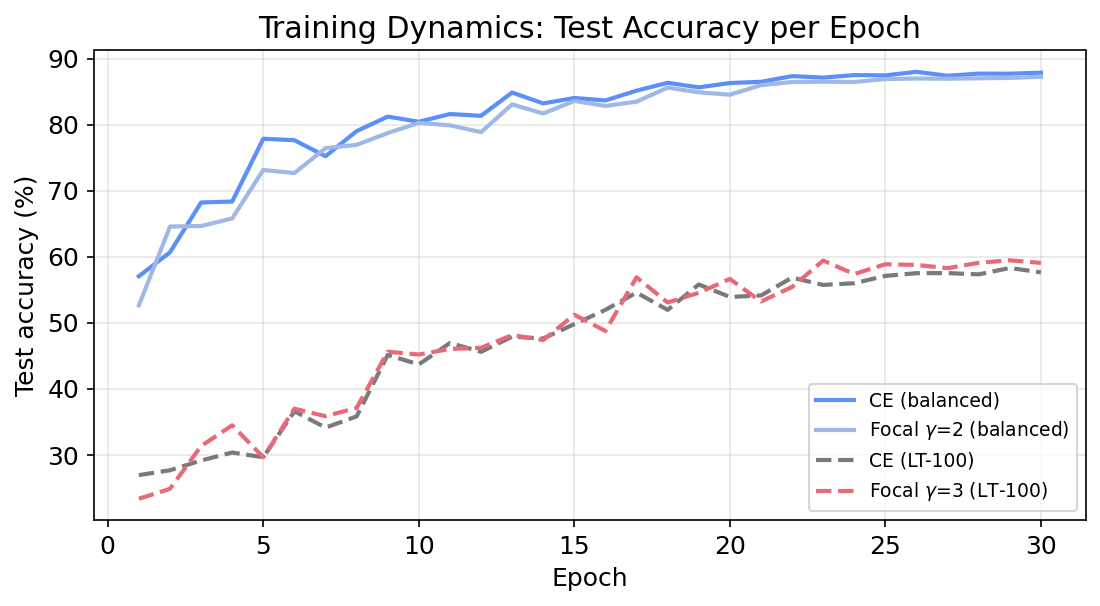
\includegraphics[width=\columnwidth]{figures/output/fig6_curves.png}
\caption{Training dynamics: test accuracy per epoch for representative configurations on both
the balanced and long-tailed settings.}
\label{fig:curves}
\end{figure}

\subsection{Discussion}
The two regimes tell a coherent story. On balanced data, every class already contributes a
similar share of easy and hard examples, so the modulating factor of focal loss mostly removes
useful gradient signal, slightly reducing accuracy; only mild focusing ($\gamma=1$) helps, and
solely by tempering overconfidence. Under heavy imbalance, the abundant head classes dominate
the cross-entropy gradient and the tail is effectively ignored, which is exactly the easy-example
dominance focal loss was built to counter. Down-weighting confident head predictions lets the
rare classes contribute, so larger $\gamma$ yields better accuracy, macro-F1, calibration, and
in particular worst-class accuracy. This matches the original motivation of focal
loss~\cite{lin2017focal} and the calibration findings of Mukhoti et
al.~\cite{mukhoti2020calibration}.

\section{Limitations and Future Work}
\label{sec:limits}
Our study fixes one architecture, one dataset family, one imbalance factor, and a single seed per
configuration, so we report point estimates rather than confidence intervals. We do not apply
temperature scaling, which is known to further improve calibration, nor do we combine focal loss
with explicit reweighting such as CB-Focal~\cite{cui2019classbalanced}. Future work should add
multiple seeds with error bars, larger backbones (e.g., ResNet), additional datasets including
ImageNet-LT, a sweep over imbalance factors, and a comparison against dedicated long-tailed
methods.

\section{Conclusion}
\label{sec:conclusion}
We asked whether focal loss beats cross-entropy for CIFAR-10 classification with a small CNN. The
answer is no on the standard balanced benchmark: cross-entropy gives the best accuracy and focal
loss helps only calibration, and only at low $\gamma$. The answer becomes yes under class
imbalance, where focal loss improves every metric and dramatically rescues rare-class accuracy,
with larger $\gamma$ preferred. Focal loss is therefore best understood as a targeted remedy for
imbalance and miscalibration rather than a generic replacement for cross-entropy. Practitioners
working with balanced data should default to cross-entropy, while those facing long-tailed
distributions should consider focal loss with a relatively large focusing parameter.

\section*{Acknowledgments}
The authors thank Vizuara AI Labs for providing mentorship and computational resources for this
research.

\begin{thebibliography}{99}
\bibitem{lin2017focal}
T.-Y. Lin, P. Goyal, R. Girshick, K. He, and P. Doll\'ar,
``Focal loss for dense object detection,''
in \textit{Proc. IEEE Int. Conf. Computer Vision (ICCV)}, 2017, pp. 2980--2988.

\bibitem{mukhoti2020calibration}
J. Mukhoti, V. Kulharia, A. Sanyal, S. Golodetz, P. H. S. Torr, and P. K. Dokania,
``Calibrating deep neural networks using focal loss,''
in \textit{Advances in Neural Information Processing Systems (NeurIPS)}, vol. 33, 2020.

\bibitem{cui2019classbalanced}
Y. Cui, M. Jia, T.-Y. Lin, Y. Song, and S. Belongie,
``Class-balanced loss based on effective number of samples,''
in \textit{Proc. IEEE Conf. Computer Vision and Pattern Recognition (CVPR)}, 2019, pp. 9268--9277.

\bibitem{cao2019ldam}
K. Cao, C. Wei, A. Gaidon, N. Arechiga, and T. Ma,
``Learning imbalanced datasets with label-distribution-aware margin loss,''
in \textit{Advances in Neural Information Processing Systems (NeurIPS)}, vol. 32, 2019.

\bibitem{guo2017calibration}
C. Guo, G. Pleiss, Y. Sun, and K. Q. Weinberger,
``On calibration of modern neural networks,''
in \textit{Proc. Int. Conf. Machine Learning (ICML)}, 2017, pp. 1321--1330.

\bibitem{buda2018systematic}
M. Buda, A. Maki, and M. A. Mazurowski,
``A systematic study of the class imbalance problem in convolutional neural networks,''
\textit{Neural Networks}, vol. 106, pp. 249--259, 2018.

\bibitem{krizhevsky2009cifar}
A. Krizhevsky,
``Learning multiple layers of features from tiny images,''
Tech. Rep., University of Toronto, 2009.

\bibitem{he2016resnet}
K. He, X. Zhang, S. Ren, and J. Sun,
``Deep residual learning for image recognition,''
in \textit{Proc. IEEE Conf. Computer Vision and Pattern Recognition (CVPR)}, 2016, pp. 770--778.

\bibitem{loshchilov2019adamw}
I. Loshchilov and F. Hutter,
``Decoupled weight decay regularization,''
in \textit{Proc. Int. Conf. Learning Representations (ICLR)}, 2019.

\bibitem{ioffe2015batchnorm}
S. Ioffe and C. Szegedy,
``Batch normalization: Accelerating deep network training by reducing internal covariate shift,''
in \textit{Proc. Int. Conf. Machine Learning (ICML)}, 2015, pp. 448--456.

\bibitem{srivastava2014dropout}
N. Srivastava, G. Hinton, A. Krizhevsky, I. Sutskever, and R. Salakhutdinov,
``Dropout: A simple way to prevent neural networks from overfitting,''
\textit{Journal of Machine Learning Research}, vol. 15, no. 1, pp. 1929--1958, 2014.

\bibitem{smith2022cyclical}
L. N. Smith,
``Cyclical focal loss,''
arXiv preprint arXiv:2202.08978, 2022.
\end{thebibliography}

\end{document}
